\documentclass[aspectratio=169,11pt,t]{beamer}

% ---------- Style: matches the Week 2 and Week 3 practice talk decks ----------
\usepackage[T1]{fontenc}
\usepackage{mathpazo}
\usepackage{helvet}
\usepackage{graphicx}
\usepackage{tikz}

\definecolor{navy}{HTML}{1F3864}
\definecolor{gold}{HTML}{F2C14E}
\definecolor{midgray}{HTML}{595959}
\definecolor{hairline}{HTML}{C8C8C8}
\definecolor{palegray}{HTML}{BFBFBF}
\definecolor{midblue}{HTML}{6E8FBF}
\definecolor{teal}{HTML}{3E7C7B}
\definecolor{grayline}{HTML}{8C8C8C}

\setbeamertemplate{navigation symbols}{}
\setbeamertemplate{itemize items}{\textcolor{navy}{\footnotesize\textbullet}}
\setbeamercolor{normal text}{fg=black}
\setbeamercolor{structure}{fg=navy}
\setbeamerfont{normal text}{family=\rmfamily}
\usefonttheme{serif}

\newcommand{\slidelabel}[1]{%
  {\sffamily\bfseries\fontsize{10}{13}\selectfont\color{navy}\MakeUppercase{#1}}\par
  \vspace{-6pt}\textcolor{hairline}{\rule{\textwidth}{0.5pt}}\par\vspace{8pt}}

\newcommand{\statlbl}[2]{%
  {\sffamily\fontsize{9}{11}\selectfont\color{midgray}\MakeUppercase{#1}}\par\vspace{6pt}
  {\sffamily\bfseries\fontsize{20}{23}\selectfont\color{navy}#2}}

% small legend swatch
\newcommand{\swatch}[2]{%
  \tikz[baseline=-0.1em,x=1pt,y=1pt]{\fill[#1] (0,-1) rectangle (8,7);}%
  \hspace{3pt}{\sffamily\fontsize{8.5}{10}\selectfont\color{midgray}#2}}

\begin{document}

% ---------- Slide 1: Title ----------
\begin{frame}
  \vspace{55pt}
  {\sffamily\fontsize{8}{11}\selectfont\color{midgray}MSDS 696 DATA SCIENCE PRACTICUM II \quad\textbar\quad WEEK 4}\par\vspace{12pt}
  {\sffamily\bfseries\fontsize{25}{30}\selectfont\color{navy}Predicting U.S. Bank Undercapitalization}\par\vspace{9pt}
  {\fontsize{12.5}{17}\selectfont\itshape\color{midgray}Comparing Four Models Against Two Benchmarks}\par\vspace{14pt}
  {\sffamily\fontsize{9.5}{13}\selectfont Oussama Ennaciri \quad\textbar\quad July 2026}\par\vspace{6pt}
  \textcolor{navy}{\rule{\textwidth}{1.2pt}}
\end{frame}

% ---------- Slide 2: Method ----------
% Column header, then evenly spaced entries beneath it.
\newcommand{\testcol}[2]{%
  {\sffamily\bfseries\fontsize{8}{10}\selectfont\color{midgray}\MakeUppercase{#1}}\par
  \vspace{3pt}\textcolor{hairline}{\rule{\linewidth}{0.4pt}}\par\vspace{9pt}
  {\fontsize{11.5}{14}\selectfont\color{navy}\setlength{\parskip}{0pt}#2\par}}
\newcommand{\testitem}[1]{#1\par\vspace{7pt}}

\begin{frame}
  \slidelabel{Method}
  \vfill
  \centerline{\begin{minipage}{0.86\textwidth}
  \begin{columns}[T,onlytextwidth]
    \begin{column}{0.46\textwidth}
      \testcol{Benchmarks}{%
        \testitem{Naive \textit{(flag every bank)}}
        \testitem{Capital ratio \textit{(distance to the 8\% threshold)}}}
    \end{column}
    \hfill
    \begin{column}{0.46\textwidth}
      \testcol{Models}{%
        \testitem{Gradient boosting}
        \testitem{Logistic regression}
        \testitem{Neural network \textit{(MLP)}}
        \testitem{Sequence network \textit{(GRU)}}}
    \end{column}
  \end{columns}
  \end{minipage}}
  \vfill
  \vspace{10pt}
\end{frame}

% ---------- Slide 3: Risky banks caught ----------
\begin{frame}
  \slidelabel{Risky banks caught}
  \vspace{4pt}
  \centering
  {\fontsize{11.5}{15}\selectfont\itshape\color{midgray}How many actually risky banks does each model rank at the top?}\par
  \vfill
  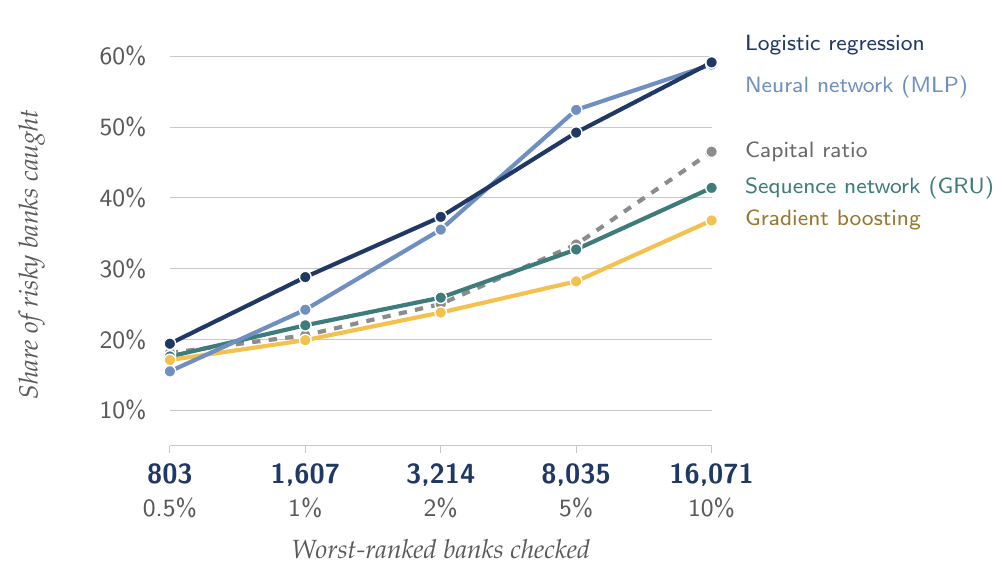
\begin{tikzpicture}[x=0.43cm,y=0.090cm,
      series/.style={line width=1.5pt,line join=round},
      dot/.style={draw=white,line width=0.5pt}]
    % plot area spans y = 5 (baseline, unlabelled) to 60
    \useasboundingbox (-4.2,-11.0) rectangle (23.8,64);

    % gridlines + y ticks
    \foreach \y in {10,20,30,40,50,60} {
      \draw[hairline,very thin] (0,\y) -- (16,\y);
      \node[left] at (-0.4,\y) {\sffamily\fontsize{9.5}{11}\selectfont\color{midgray}\y\%};
    }
    \draw[hairline] (0,5) -- (16,5);

    % y-axis title, centred on the plot area
    \node[rotate=90,anchor=south] at (-3.4,32) {\itshape\fontsize{9.5}{12}\selectfont\color{midgray}Share of risky banks caught};

    % x ticks: two rows, count then share
    \foreach \x/\pct/\n in {0/0.5\%/803, 4/1\%/1{,}607, 8/2\%/3{,}214, 12/5\%/8{,}035, 16/10\%/16{,}071} {
      \draw[hairline] (\x,5) -- (\x,4.0);
      \node[anchor=north] at (\x,3.8) {\sffamily\bfseries\fontsize{10}{12}\selectfont\color{navy}\n};
      \node[anchor=north] at (\x,-1.0) {\sffamily\fontsize{9}{11}\selectfont\color{midgray}\pct};
    }
    % x-axis title, matching the y-axis title
    \node[anchor=north] at (8,-6.8) {\itshape\fontsize{9.5}{12}\selectfont\color{midgray}Worst-ranked banks checked};

    % series
    \draw[series,grayline,dashed] (0,18.1) -- (4,20.6) -- (8,25.0) -- (12,33.4) -- (16,46.5);
    \draw[series,teal]            (0,17.6) -- (4,22.0) -- (8,25.9) -- (12,32.7) -- (16,41.4);
    \draw[series,gold]            (0,17.1) -- (4,19.9) -- (8,23.8) -- (12,28.2) -- (16,36.8);
    \draw[series,midblue]         (0,15.5) -- (4,24.2) -- (8,35.5) -- (12,52.4) -- (16,58.8);
    \draw[series,navy]            (0,19.4) -- (4,28.8) -- (8,37.3) -- (12,49.2) -- (16,59.1);

    % point markers
    \foreach \x/\y in {0/18.1,4/20.6,8/25.0,12/33.4,16/46.5} \fill[grayline,dot] (\x,\y) circle (2.1pt);
    \foreach \x/\y in {0/17.6,4/22.0,8/25.9,12/32.7,16/41.4} \fill[teal,dot]     (\x,\y) circle (2.1pt);
    \foreach \x/\y in {0/17.1,4/19.9,8/23.8,12/28.2,16/36.8} \fill[gold,dot]     (\x,\y) circle (2.1pt);
    \foreach \x/\y in {0/15.5,4/24.2,8/35.5,12/52.4,16/58.8} \fill[midblue,dot]  (\x,\y) circle (2.1pt);
    \foreach \x/\y in {0/19.4,4/28.8,8/37.3,12/49.2,16/59.1} \fill[navy,dot]     (\x,\y) circle (2.1pt);

    % direct labels at the right end, nudged apart where lines converge
    \node[anchor=west] at (16.7,61.6) {\sffamily\fontsize{8.5}{10}\selectfont\color{navy}Logistic regression};
    \node[anchor=west] at (16.7,55.6) {\sffamily\fontsize{8.5}{10}\selectfont\color{midblue}Neural network (MLP)};
    \node[anchor=west] at (16.7,46.5) {\sffamily\fontsize{8.5}{10}\selectfont\color{grayline!75!black}Capital ratio};
    \node[anchor=west] at (16.7,41.4) {\sffamily\fontsize{8.5}{10}\selectfont\color{teal}Sequence network (GRU)};
    \node[anchor=west] at (16.7,36.8) {\sffamily\fontsize{8.5}{10}\selectfont\color{gold!62!black}Gradient boosting};
  \end{tikzpicture}
  \vfill
\end{frame}

\end{document}
